\PassOptionsToPackage{svgnames}{xcolor}
\documentclass{article}
\usepackage{sectsty}% http://ctan.org/pkg/sectsty
\usepackage{xcolor}% http://ctan.org/pkg/xcolor
\sectionfont{\color{cyan}}
\usepackage{graphicx}
\usepackage{lipsum}\usepackage{biblatex}
\usepackage{multicol}\usepackage{xcolor}
\usepackage{array}
\usepackage{pgf}  
\usepackage{tcolorbox}
\usepackage{tcolorbox}
\tcbuselibrary{most}
\usepackage{lipsum}
\tcbuselibrary{skins,breakable}
\usetikzlibrary{shadings,shadows}
\usepackage{float}
\definecolor{ultramarine1}{rgb}{0.07, 0.04, 0.56} 
\usepackage{mathtools}  \usepackage{nopageno}
\usepackage{amsmath, amsthm, amssymb, amsfonts}
\usepackage{exscale}\usepackage{lmodern}
\usepackage{xcolor}
\usepackage{ushort}
\usepackage{setspace}%\usepackage[x11names]{xcolor}
\usepackage{url}

\usepackage[paperwidth=297mm,paperheight=420mm,left=0.5in,right=0.5in,top=5.5cm,bottom=0.5in]{geometry}
\setlength\columnsep{1cm} 

\AddToHook{shipout/background}{%
	\put (0in,-\paperheight){
\includegraphics[width=\paperwidth,height=\paperheight]{fundo_ermac1}}%

}
%%%%%%%%%%%%%%%%%
\newenvironment{myexampleblock}[1]{%
	\tcolorbox[beamer,%
	noparskip,breakable,
	colback=LightGreen,colframe=DarkGreen,%
	colbacklower=LimeGreen!75!LightGreen,%
	title=#1]}%
{\endtcolorbox}

\newenvironment{myalertblock}[1]{%
	\tcolorbox[beamer,%
	noparskip,breakable,
	colback=LightCoral,colframe=DarkRed,%
	colbacklower=Tomato!75!LightCoral,%
	title=#1]}%
{\endtcolorbox}

\newenvironment{myblock}[1]{%
	\tcolorbox[beamer,%
	noparskip,breakable,
	colback=Grey!20,colframe=Grey!25,%
	colbacklower=White,%
	title=#1]}%
{\endtcolorbox}

\newtcolorbox{question}{breakable,colframe=cyan!40,colback=cyan!10}

%%%%%%%%%%%%%%%%%%%%%%%%%%%%%%%%%%%%%%%%%%%%%%%%%%%
%
%
%
%
%%%%%%%%%%%%%%%%%%%%%%%%%%%%%%%%%%%%%%%%%%%%%%%%%%%
\begin{document} 
	
	{\fontsize{30}{38} \selectfont \noindent \textbf{Title of the Poster}} \vspace{0.4cm}\\
	{\fontsize{15}{23} \selectfont {Author 1, Author 2}\\
	{\fontsize{12}{20} \selectfont {{Indian Institute of Space Science and Technology, Thiruvananthapuram}
	%%%%%%%%%%%%%%%%%%%%%%%%%%%%%%%%%%%%%%%%%%%%%%%%%%%%
	\begin{multicols}{2}
		
			\noindent\begin{minipage}[t][.78\textheight][t]{\columnwidth}
				\section*{\Huge{\textcolor{cyan}{Introduction}}}
				% Add introduction replacing lipsum
				\lipsum[1]
				
				\section*{\Huge{\textcolor{cyan}{Objective}}}
				\lipsum[1]
				
				\section*{\Huge{\textcolor{cyan}{Methodology}}}
				Lorem Ipsum is simply dummy text of the printing and typesetting industry. Lorem Ipsum has been the industry's standard dummy text ever since the 1500s, when an unknown printer took a galley of type and scrambled it to make a type specimen book. It has survived not only five centuries, but also the leap into electronic
			\end{minipage}
			
			\columnbreak
			
			\noindent\begin{minipage}[t][.78\textheight][t]{\columnwidth}
				\section*{\Huge{\textcolor{cyan}{Results}}}
				% Add results below
				\lipsum[1-1] 
				
				
				\begin{figure}[H]\centering
					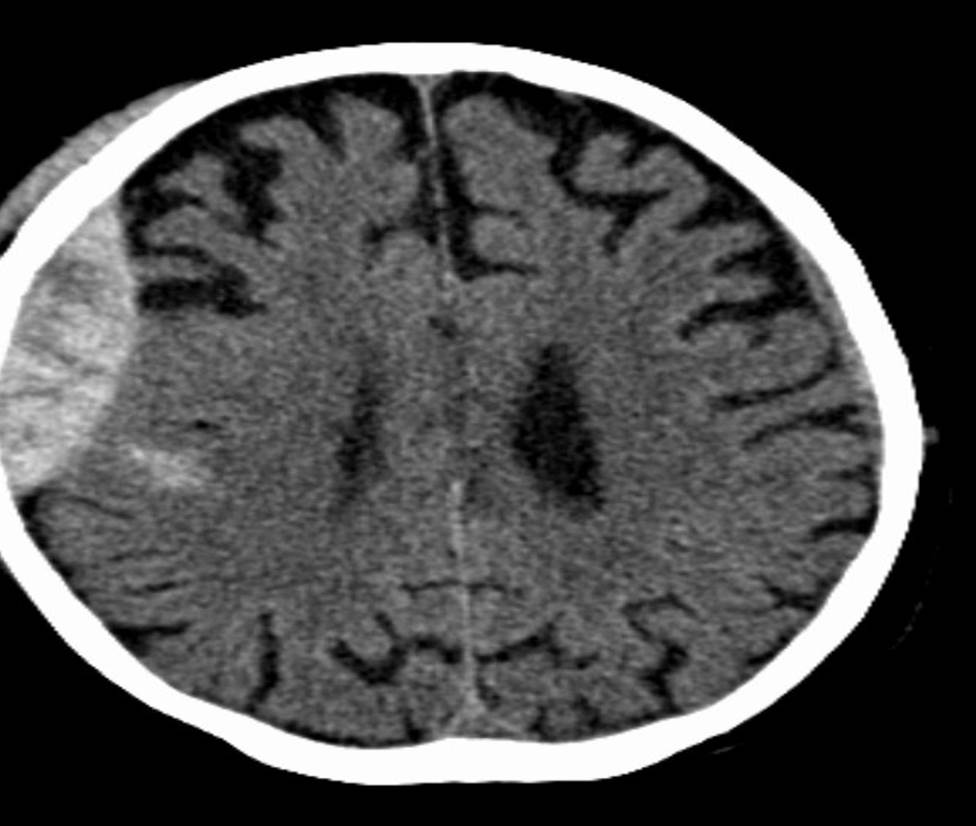
\includegraphics[width=5cm]{Bild3}
				\end{figure}
			
			
			\section*{\Huge{\textcolor{cyan}{Conclusion}}}
			Lorem Ipsum is simply dummy text of the printing and typesetting industry. Lorem Ipsum has been the industry's standard dummy text ever since the 1500s, when an unknown printer took a galley of type and scrambled it to make a type specimen book. It has survived not only five centuries, but also the leap into electronic
			\end{minipage}
		
	\end{multicols}

\vspace{-0.5cm}
\textcolor{ultramarine1}{\hspace{-0.8cm}\rule{28cm}{1pt}}\vspace{-0.25cm}
\begin{multicols}{2}
	
	\vspace{-0.2cm}\noindent\begin{minipage}[t][.12\textheight][t]{\columnwidth}
		
		\begin{question}
			\section*{Contacts}
		e-mail Author 1:.................\\
		e-mail Author 2: ................
		
		\end{question}
	\end{minipage}
	
	\columnbreak
	
	\noindent\begin{minipage}[t][.12\textheight][t]{\columnwidth}
		
		\begin{thebibliography}{9}
			\bibitem{texbook}
			Donald E. Knuth (1986) \emph{The \TeX{} Book}, Addison-Wesley Professional.
			\bibitem{lamport94}
			Leslie Lamport (1994) \emph{\LaTeX: a document preparation system}, Addison
			Wesley, Massachusetts, 2nd ed.
		\end{thebibliography}
		
	\end{minipage}
	
\end{multicols}



\end{document}